\section{Results}
\label{sec:results}
\subsection{OE scores below PPO-DR during adaptation}
OE performs below PPO-DR, contrary to the primary prediction. Across T2 and T3, OE has a pooled AUC IQM of $0.2905$, compared with $0.8497$ for PPO-DR. Their difference is $-0.5592$ with a nominal 95\% interval of $[-0.6088,-0.5196]$, entirely below the negative margin. OE also scores below ES-DR in the prespecified S1 comparison: the IQM difference is $-0.5871$ and the Holm-adjusted rank-test $p$ value is $0.00110$. Figure~\ref{fig:primary} shows estimates for all six procedures.

\begin{figure}[tb]
\centering
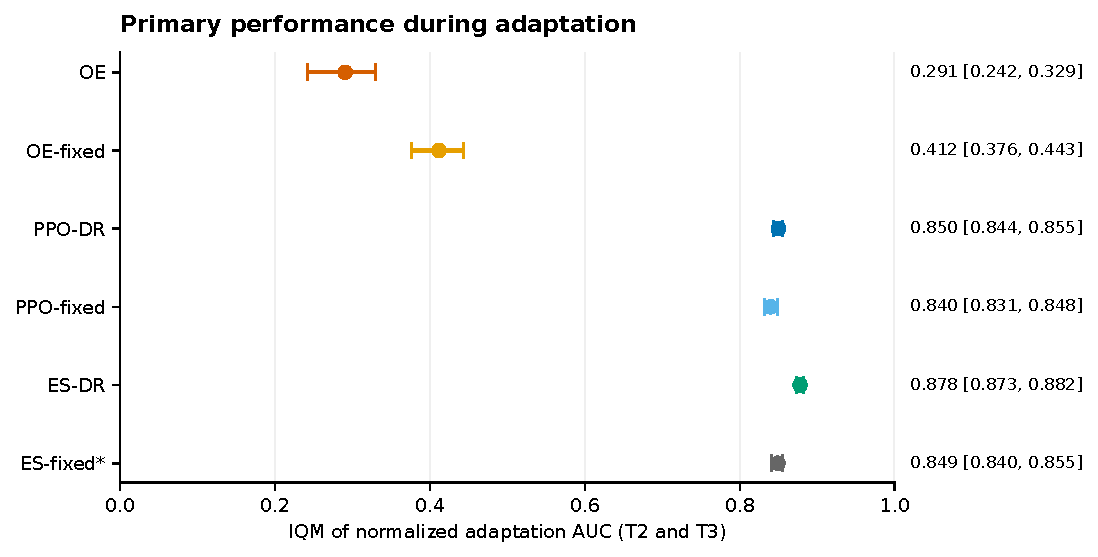
\includegraphics[width=0.92\linewidth]{figures/fig02_primary.pdf}
\caption{\textbf{Performance during adaptation on T2 and T3.} Points show pooled IQMs of normalized AUC; bars are nominal 95\% whole-run percentile bootstrap intervals from 50,000 draws. Each procedure has ten training runs evaluated on twenty fixed environments. Asterisk: ES-fixed was added after the core experiment.}
\label{fig:primary}
\end{figure}

OE is already below PPO-DR before adaptation. The zero-shot IQM difference on T2/T3 is $-0.4648$; at the final checkpoint it is $-0.6035$ (S4 and S5, both Holm-adjusted $p=0.00110$). Figure~\ref{fig:curves} shows the mean trajectories. In T2, OE's mean normalized competence declines from $0.4383$ to $0.2338$, while PPO-DR changes from $0.7244$ to $0.7478$. T3 shows a smaller decline for OE, from $0.2966$ to $0.2655$.

On the in-range T1 suite, the OE--PPO-DR difference in adaptation AUC is $-0.5371$ (nominal 95\% interval $[-0.5951,-0.4799]$; S6). 

\subsection{Fixed and varied training}
The separately tuned varied OE procedure scores below OE-fixed on T2/T3 AUC: difference $-0.1210$, interval $[-0.1799,-0.0680]$ (S2; Holm-adjusted $p=0.00440$). For PPO, the corresponding difference is $0.0099$, interval $[-0.0004,0.0201]$. Its predicted direction is unsupported under the prespecified rank-test rule (S3; adjusted $p=0.6232$).

In the later ES-fixed extension, ES-DR has higher T2/T3 adaptation AUC by $0.0286$ (nominal 95\% interval $[0.0203,0.0384]$), below the $0.05$ margin. The corresponding rank test gives adjusted $p=0.000365$. ES-DR also has higher T1 zero-shot competence by $0.0645$ (interval $[0.0499,0.0788]$; adjusted $p=0.000365$).

Selected hyperparameters also differ between fixed and varied configurations. For OE, the mutation standard deviation is $0.03412$ under varied training and $0.00507$ under fixed training.

\begin{figure}[tb]
\centering
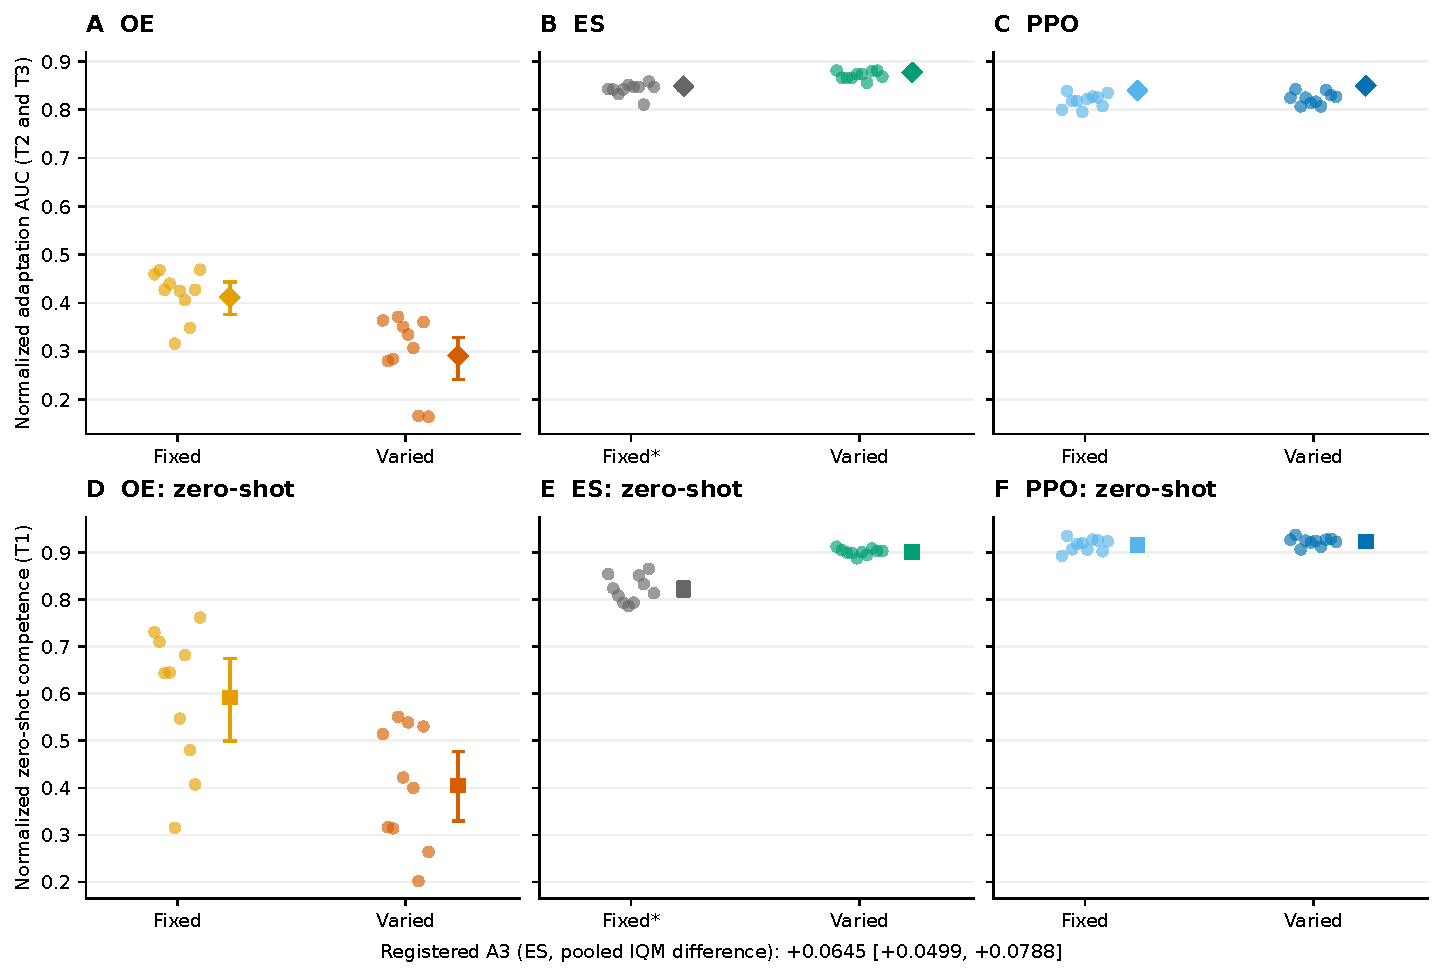
\includegraphics[width=\linewidth]{figures/fig03_variation.pdf}
\caption{\textbf{Fixed and varied configurations.} Upper panels: T2/T3 AUC, with run means (circles), pooled IQMs (diamonds) and nominal 95\% whole-run intervals. Lower panels: T1 zero-shot run means and their mean (squares), with descriptive 95\% intervals from 20,000 whole-run bootstrap draws. A3 denotes the pooled-IQM contrast; lower OE/PPO panels are descriptive. Each configuration was tuned separately. Asterisk: ES-fixed extension.}
\label{fig:variation}
\end{figure}

\subsection{Population persistence and support}
OE has higher extinction in the separate persistence assay than PPO-DR. Across T2/T3, the S7 difference in IQMs of per-run extinction fractions is $0.3750$, interval $[0.2500,0.4833]$, against the predicted OE advantage (adjusted $p=0.00110$). Table~\ref{tab:persistence} reports the descriptive extinction frequencies for every procedure. Extinction is frequent across all six procedures in resource-scarce T2, including those with high normalized competence. High relative food acquisition can coexist with insufficient intake for population survival.

\begin{table}[tb]
\centering\small
\caption{Descriptive extinction frequencies in the separate 5,000-step no-floor assay. Each cell pools ten runs across ten fixed environments; these 100 observations are not independent training runs.}\label{tab:persistence}
\begin{tabularx}{\linewidth}{lYYY}
\toprule
Procedure & T1 & T2 & T3\\\midrule
OE & 0.48 & 0.94 & 0.76\\
OE-fixed & 0.30 & 0.93 & 0.48\\
PPO-DR & 0.03 & 0.83 & 0.15\\
PPO-fixed & 0.10 & 0.95 & 0.14\\
ES-DR & 0.03 & 0.89 & 0.22\\
ES-fixed* & 0.11 & 0.87 & 0.21\\
\bottomrule
\end{tabularx}
\end{table}


The population floor makes a substantial contribution during OE training and adaptation. The mean run-level share of training births supplied by the floor is approximately $58\%$ for OE and $59\%$ for OE-fixed. During T2 adaptation, the pooled shares rise to $99.53\%$ and $99.60\%$, respectively (Table~\ref{tab:floor}).

\begin{table}[tb]
\centering\small
\caption{Share of new agents supplied by population-floor replacements during adaptation. Fractions pool event counts over ten runs and ten environments per suite.}\label{tab:floor}
\begin{tabularx}{\linewidth}{lYY}
\toprule
Suite & OE & OE-fixed\\\midrule
T1 & 64.35\% & 59.29\%\\
T2 & 99.53\% & 99.60\%\\
T3 & 78.90\% & 71.87\%\\
\bottomrule
\end{tabularx}
\end{table}


\subsection{Learning curves}
Between the first validation checkpoint near 20 million steps and the end of training at 200 million steps, OE's mean score above random increases from $9.4818$ to $10.6102$; six of ten runs improve (Figure~\ref{fig:curves}). Three additional exploratory runs extend OE training to one billion steps (Appendix~\ref{app:diagnostics}).

\begin{figure}[!t]
\centering
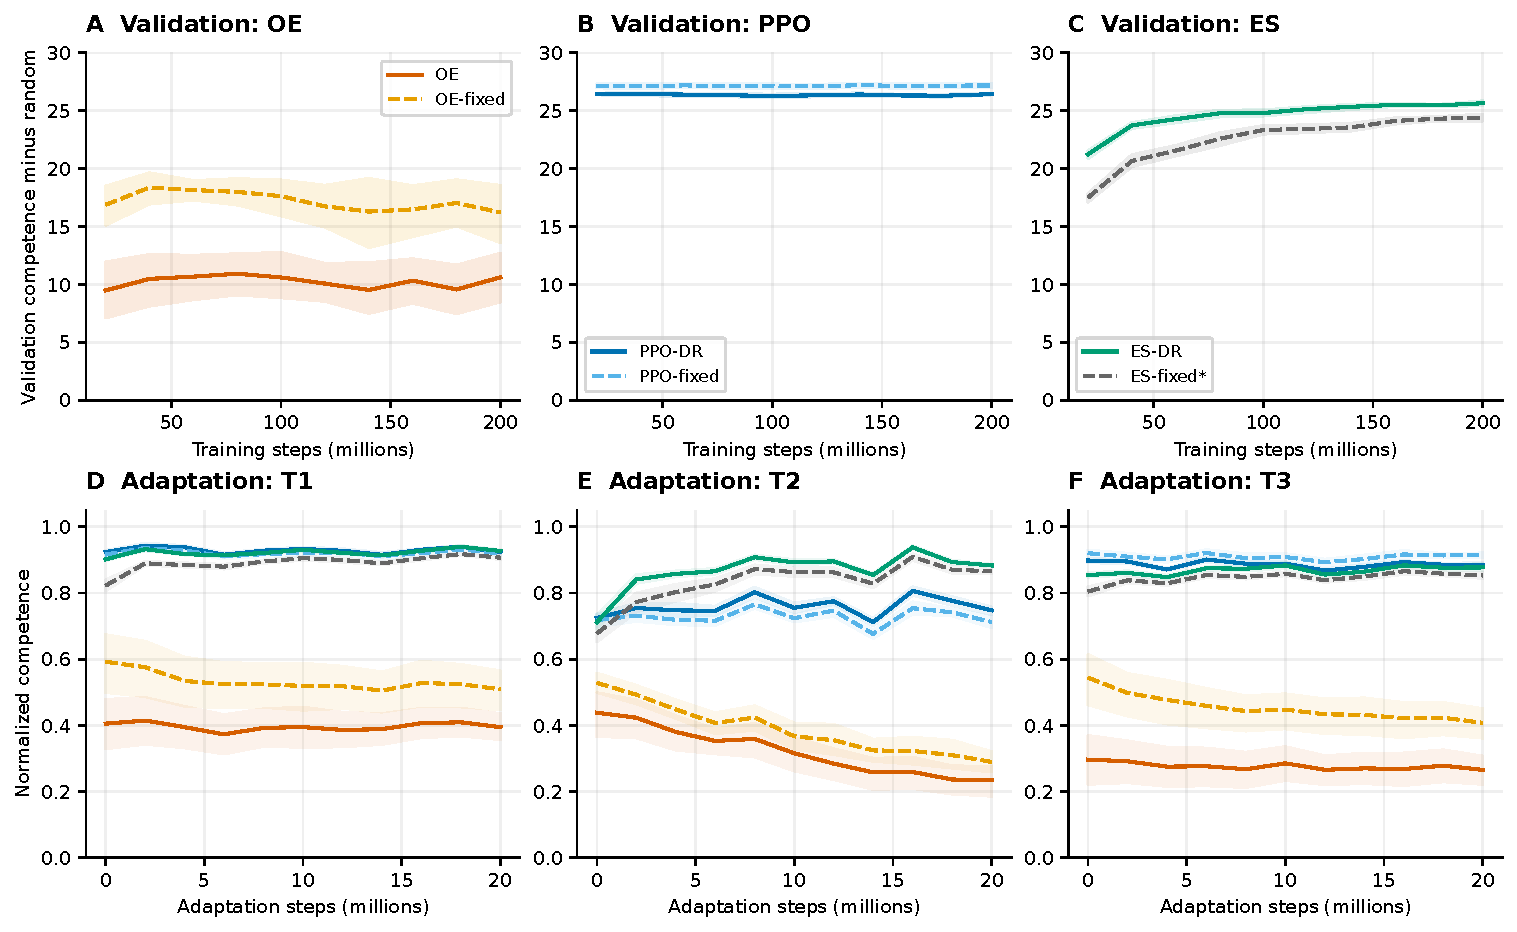
\includegraphics[width=\linewidth]{figures/fig04_curves.pdf}
\caption{\textbf{Training and adaptation.} Upper panels: validation competence above the random reference. Lower panels: normalized test competence during adaptation. Lines average ten runs; shading gives pointwise 95\% whole-run percentile intervals from 20,000 draws. Axes use nominal living-agent steps. Training measurements begin near 20 million steps.}
\label{fig:curves}
\end{figure}

The OE--PPO-DR contrast remains negative under paired-seed resampling, re-estimation of normalization anchors and integration over actual step counts. The weaker PPO fixed/varied comparison depends on the summary and resampling method (Appendix~\ref{app:diagnostics}).
